\documentclass[12pt,a4paper]{article}

% ─── Packages ───────────────────────────────────────────────────────────────
\usepackage[margin=2.5cm]{geometry}
\usepackage{amsmath,amssymb,amsthm}
\usepackage{graphicx}
\usepackage{booktabs}
\usepackage{array}
\usepackage{hyperref}
\usepackage{xcolor}
\usepackage{caption}
\usepackage{subcaption}
\usepackage{enumitem}
\usepackage{float}
\usepackage{tabularx}
\usepackage{multirow}
\usepackage{setspace}
\usepackage{fancyhdr}
\usepackage{titlesec}
\usepackage{parskip}
\usepackage{tikz}
\usepackage{tcolorbox}
\usepackage{microtype}
\usepackage{cleveref}
\usepackage{soul}
\usepackage{mdframed}
\usetikzlibrary{shapes.geometric, arrows.meta, positioning, fit, backgrounds, calc}

% ─── Colour Palette ─────────────────────────────────────────────────────────
\definecolor{apblue}{RGB}{30,90,160}
\definecolor{apgold}{RGB}{204,153,0}
\definecolor{aplightblue}{RGB}{220,235,250}
\definecolor{apgrey}{RGB}{245,245,245}
\definecolor{apdarkgrey}{RGB}{80,80,80}
\definecolor{apgreen}{RGB}{0,128,80}
\definecolor{aporange}{RGB}{210,100,0}

% ─── Hyperref Setup ─────────────────────────────────────────────────────────
\hypersetup{
    colorlinks=true,
    linkcolor=apblue,
    citecolor=apgreen,
    urlcolor=apblue,
    pdftitle={Proactive Access Point Load Prediction using Temporal and Spatial Features},
    pdfauthor={Team 5 – Cupcake},
    pdfkeywords={wireless networks, access point, TCN, GNN, congestion prediction},
}

% ─── tcolorbox styles ────────────────────────────────────────────────────────
\tcbuselibrary{skins,breakable}
\newtcolorbox{insightbox}[1][]{
    enhanced,
    colback=aplightblue,
    colframe=apblue,
    fonttitle=\bfseries\color{apblue},
    title=Key Insight,
    left=6pt, right=6pt, top=4pt, bottom=4pt,
    boxrule=1pt,
    #1
}
\newtcolorbox{notebox}[1][]{
    enhanced,
    colback=apgrey,
    colframe=apdarkgrey,
    left=6pt, right=6pt, top=3pt, bottom=3pt,
    boxrule=0.5pt,
    #1
}

% ─── Page Style ─────────────────────────────────────────────────────────────
\pagestyle{fancy}
\fancyhf{}
\rhead{\textcolor{apdarkgrey}{\small Wireless Networks – Team 5 (Cupcake)}}
\lhead{\textcolor{apblue}{\small\textbf{PredictiveAP}}}
\rfoot{\thepage}
\renewcommand{\headrulewidth}{0.6pt}
\renewcommand{\headrule}{\hbox to\headwidth{\color{apblue}\leaders\hrule height \headrulewidth\hfill}}

% ─── Section Formatting ─────────────────────────────────────────────────────
\titleformat{\section}
    {\large\bfseries\color{apblue}}
    {\thesection.}{0.6em}{}
    [\vspace{-0.5em}\textcolor{apblue}{\rule{\linewidth}{1.2pt}}]

\titleformat{\subsection}
    {\normalsize\bfseries\color{apblue!80!black}}
    {\thesubsection.}{0.5em}{}

\titleformat{\subsubsection}
    {\normalsize\itshape\color{apdarkgrey}}
    {\thesubsubsection.}{0.5em}{}

\titlespacing*{\section}{0pt}{14pt}{6pt}
\titlespacing*{\subsection}{0pt}{10pt}{4pt}
\titlespacing*{\subsubsection}{0pt}{8pt}{2pt}

% ─── Caption Styling ────────────────────────────────────────────────────────
\captionsetup{
    font=small,
    labelfont={bf,color=apblue},
    labelsep=period,
    format=hang,
}

% ─── Misc Helpers ────────────────────────────────────────────────────────────
\newcommand{\code}[1]{\texttt{\small#1}}
\newcommand{\ttc}{\textsc{TTC}}
\newcommand{\predap}{\textbf{PredictiveAP}}

% ─── Title ──────────────────────────────────────────────────────────────────
\title{
    \vspace{-1.2cm}
    {\color{apblue}\rule{\linewidth}{2pt}}\\[0.6em]
    \Large\textbf{\predap: Proactive Access Point Load Prediction}\\[0.35em]
    \large Using Temporal and Spatial Deep Learning Approaches\\[0.8em]
    \normalsize\textcolor{apdarkgrey}{Wireless Networks Coursework Report\enspace$\bullet$\enspace IIITDM Kancheepuram}\\[0.2em]
    {\color{apblue}\rule{\linewidth}{1pt}}
}

\author{
    \textbf{Team 5 – Cupcake}\\[0.5em]
    \begin{tabular}{cc}
        Shishir \textcolor{apdarkgrey}{\small(CS23B2043)} & Revanth Kolla \textcolor{apdarkgrey}{\small(CS23B1085)}\\[2pt]
        Sohan \textcolor{apdarkgrey}{\small(CS23B1004)}   & Sevith Illa \textcolor{apdarkgrey}{\small(CS23I1041)}
    \end{tabular}
}
\date{\textcolor{apdarkgrey}{April 2026}}

% ════════════════════════════════════════════════════════════════════════════
\begin{document}

\maketitle
\thispagestyle{empty}
\vspace{0.3em}

% ─── Abstract ───────────────────────────────────────────────────────────────
\begin{tcolorbox}[
    enhanced,
    colback=apgrey,
    colframe=apblue,
    title=\textbf{Abstract},
    fonttitle=\color{white},
    coltitle=white,
    attach boxed title to top left={yshift=-2mm,xshift=6mm},
    boxed title style={colback=apblue},
    left=6pt, right=6pt, top=10pt, bottom=6pt,
    boxrule=1pt,
]
Wireless network congestion is a persistent challenge in dense deployment environments such as enterprise campuses and public venues. Reactive management strategies — which respond only after congestion has already occurred — lead to degraded user experience and suboptimal resource utilisation. In this work, we present \predap, a framework for proactive access point (AP) load prediction via regression on \emph{Time-to-Congestion} (\ttc). We design and evaluate three modelling approaches on a hybrid dataset derived from real CRAWDAD Wi-Fi traces and synthetic congestion scenarios.
\medskip

\textbf{Approach A} employs a Temporal Convolutional Network (TCN) with Monte Carlo Dropout to produce calibrated uncertainty estimates. \textbf{Approach B} provides a conformal prediction baseline using traditional machine learning. \textbf{Approach C} extends the feature space with graph-based spatial enrichment (GNN-lite) and an XGBoost ensemble, complemented by SHAP interpretability and ablation analysis.
\medskip

Our key finding is that \textbf{temporal features dominate predictive performance}: spatial neighbour information provides negligible additional signal on this dataset, a result confirmed both by ablation study and SHAP analysis. The TCN model achieves the best accuracy (\(\text{MAE} \approx 0.45\) intervals, \(R^2 \approx 0.71\)) with interpretable uncertainty bounds.
\end{tcolorbox}

\vspace{0.5em}
\tableofcontents
\newpage

% ════════════════════════════════════════════════════════════════════════════
\section{Introduction}
\label{sec:intro}

The proliferation of Wi-Fi-connected devices — from smartphones and laptops to IoT sensors — has made access point (AP) load management a critical concern for network operators. When an AP becomes congested, all associated clients experience degraded throughput, increased latency, and dropped connections. Traditional network management systems address congestion \emph{reactively}: a handover or load-balancing action is triggered only once the network is already saturated. This reactive paradigm is fundamentally limited, because by the time congestion is detected, service quality has already deteriorated.

A more principled approach is \emph{proactive} management: predict impending congestion with sufficient lead time so the controller can take corrective action — such as load balancing, soft handover, or rate control — \emph{before} the threshold is crossed. This requires accurate, timely regression of how long until a given AP is expected to become congested, which we formulate as the \textbf{Time-to-Congestion (\ttc)} target.

This project, \predap, investigates whether deep learning architectures that exploit the \emph{temporal} dynamics of client arrivals and departures can accurately predict \ttc. We further investigate whether incorporating \emph{spatial} information — load patterns of neighbouring APs obtained via a lightweight graph neural network layer — provides additional benefit. The answers to these questions have direct implications for the design of next-generation proactive wireless controllers.

\medskip
\noindent\textbf{Summary of Contributions:}
\begin{itemize}[noitemsep, topsep=4pt]
    \item Construction of a hybrid Wi-Fi dataset combining real CRAWDAD traces with synthetic high-load events, ensuring sufficient congestion examples for training.
    \item Implementation of three complementary \ttc\ regression approaches, each with a distinct uncertainty quantification mechanism.
    \item Rigorous ablation and SHAP analysis empirically revealing the dominance of temporal over spatial features, a result with direct implications for controller design.
    \item A practical foundation for embedding proactive prediction into a network controller simulation loop.
\end{itemize}

% ════════════════════════════════════════════════════════════════════════════
\section{Literature Survey and Research Gaps}
\label{sec:litsurvey}

\subsection{Traditional Reactive Network Management}

Classical wireless network management relies on threshold-based trigger systems. When an AP's client count exceeds a predefined capacity, or when RSSI drops below a threshold, a handover or load-balancing action is initiated~\cite{3gpp_ts36}. While straightforward to implement, these approaches are insensitive to rising load trends and cannot differentiate between transient spikes and sustained overloads — they act only \emph{post-hoc}.

\subsection{Machine Learning for Wireless Prediction}

The application of machine learning to Wi-Fi and cellular network prediction has grown substantially. Time-series models such as LSTMs~\cite{hochreiter1997lstm} and Temporal Convolutional Networks~\cite{bai2018tcn} have demonstrated strong performance on cellular traffic prediction. XGBoost~\cite{chen2016xgboost} and gradient-boosted ensembles have been applied to AP selection and user churn. Graph Neural Networks~\cite{kipf2017gcn} have been proposed for modelling spatial dependencies between base stations in heterogeneous networks.

\subsection{Identified Research Gaps}

Despite this body of work, several gaps remain unaddressed in the context of per-AP \ttc\ regression:

\begin{table}[H]
\centering
\caption{Research Gaps and How This Project Addresses Them}
\label{tab:gaps}
\renewcommand{\arraystretch}{1.35}
\begin{tabular}{>{\bfseries\color{apblue}}l p{9cm}}
\toprule
\textbf{Gap} & \textbf{Description and Our Mitigation} \\
\midrule
Gap 1 & \textbf{Lack of temporal modelling.} Prior approaches typically use instantaneous features, ignoring load trajectory. \textit{Addressed by: TCN sequence modelling (Approach A).} \\[4pt]
Gap 2 & \textbf{No uncertainty awareness.} Predictions are point estimates with no confidence signal, leading to over/under-reaction. \textit{Addressed by: MC Dropout (A) and conformal wrapping (B).} \\[4pt]
Gap 3 & \textbf{Weak robustness.} Models are trained on clean operational data and untested under congestion spikes. \textit{Addressed by: synthetic data augmentation.} \\[4pt]
Gap 4 & \textbf{Unverified spatial dependency.} Many works assume inter-AP spatial correlation, but this is rarely validated empirically. \textit{Addressed by: ablation and SHAP analysis (Approach C).} \\
\bottomrule
\end{tabular}
\end{table}

% ════════════════════════════════════════════════════════════════════════════
\section{Dataset and Feature Engineering}
\label{sec:dataset}

\subsection{Data Sources and Hybrid Strategy}

We use a \textbf{hybrid dataset} combining two complementary sources:

\subsubsection{Real Data: CRAWDAD Wi-Fi Traces}
The CRAWDAD repository provides real-world Wi-Fi syslog data from university campus deployments. We parse three merged syslog files covering three days of operation (60,000+ client events). Key information extracted includes client association/disassociation events, AP identifiers, and timestamps. This yields authentic temporal access patterns under realistic load conditions.

\subsubsection{Synthetic Data: Congestion Simulation}
Real CRAWDAD data alone is insufficient for training a \ttc\ regression model because organic congestion events are rare and unevenly distributed. We therefore generate \textbf{synthetic high-load intervals} by injecting artificial client spikes into the real time series, parameterised by empirically observed load patterns, ensuring the training and validation sets contain sufficient examples of APs approaching and exceeding their capacity limits.

The final temporally-ordered splits are as follows: Train ($\approx$19,500 samples), Validation ($\approx$7,500 samples), and Test (318 held-out samples). All splits are strictly chronological to prevent temporal data leakage.

\subsection{Target Variable: Time-to-Congestion (\ttc)}

For each AP at each 30-second aggregation window, \ttc\ is computed as the number of future intervals until the AP's client count crosses the predefined congestion threshold. \ttc\ ranges from 0 (already congested) to 60 (comfortably below threshold). Rows where \ttc\ cannot be computed are dropped.

\subsection{Feature Engineering}

Features are grouped into three categories, as summarised in \Cref{tab:features}.

\begin{table}[H]
\centering
\caption{Feature Groups Used for \ttc\ Prediction}
\label{tab:features}
\renewcommand{\arraystretch}{1.35}
\begin{tabular}{>{\bfseries}l l p{6.5cm}}
\toprule
\textbf{Group} & \textbf{Feature} & \textbf{Description} \\
\midrule
\multirow{4}{*}{\color{apblue}Temporal} 
 & \code{hour\_of\_day} & Hour within the day (0–23); captures daily activity cycles \\
 & \code{day\_of\_week} & Day of the week (0–6); captures weekly periodicity \\
 & \code{clients\_lag1/lag2} & Client count at $t{-}1$ and $t{-}2$; direct load memory \\
 & \code{clients\_roll5\_mean/std} & Rolling 5-step mean and std dev; trend smoothing \\
\midrule
\multirow{2}{*}{\color{aporange}Dynamic} 
 & \code{clients\_connected} & Current number of associated clients \\
 & \code{clients\_delta} & Change in client count from previous step \\
\midrule
\multirow{2}{*}{\color{apgreen}Spatial}
 & \code{neighbor\_avg\_load} & Average client load of neighbouring APs \\
 & \code{channel\_utilization} & Estimated channel utilisation \\
\bottomrule
\end{tabular}
\end{table}

\begin{notebox}
\textbf{Preprocessing:} Features are Z-score normalised using scalers fit exclusively on the training split. The \ttc\ target is $\log_{1p}$ transformed to reduce right-skew, then Z-score normalised; predictions are inverse-transformed for evaluation.
\end{notebox}

% ════════════════════════════════════════════════════════════════════════════
\section{Methodology}
\label{sec:methodology}

We implement three distinct approaches to \ttc\ regression. Each targets a different research gap identified in \Cref{tab:gaps}, and together they form a progressive stack from deep temporal modelling through to spatial enrichment and interpretability.

% ─── Approach A ──────────────────────────────────────────────────────────────
\subsection{Approach A — Temporal Convolutional Network with MC Dropout}
\label{subsec:approach_a}

\subsubsection{Motivation}
Approach A directly addresses Gaps 1 and 2: temporal modelling and uncertainty quantification. Dilated 1D convolutions in a TCN can model long-range temporal dependencies efficiently and in parallel, avoiding the vanishing gradients and sequential computation bottlenecks of recurrent architectures.

\subsubsection{Sequence Construction}
For each AP, we build a sliding window of $L = 20$ consecutive time steps (representing 10 minutes of history). Each window is a tensor of shape $(20, 11)$ — 20 steps across 11 features. The label is the scaled \ttc\ at the last time step of the window.

\subsubsection{Architecture}

\begin{figure}[H]
    \centering
    % ── PLACEHOLDER: Replace with your actual architecture diagram ──
    % Suggested tool: draw.io or TikZ. See Section 7 for specs.
    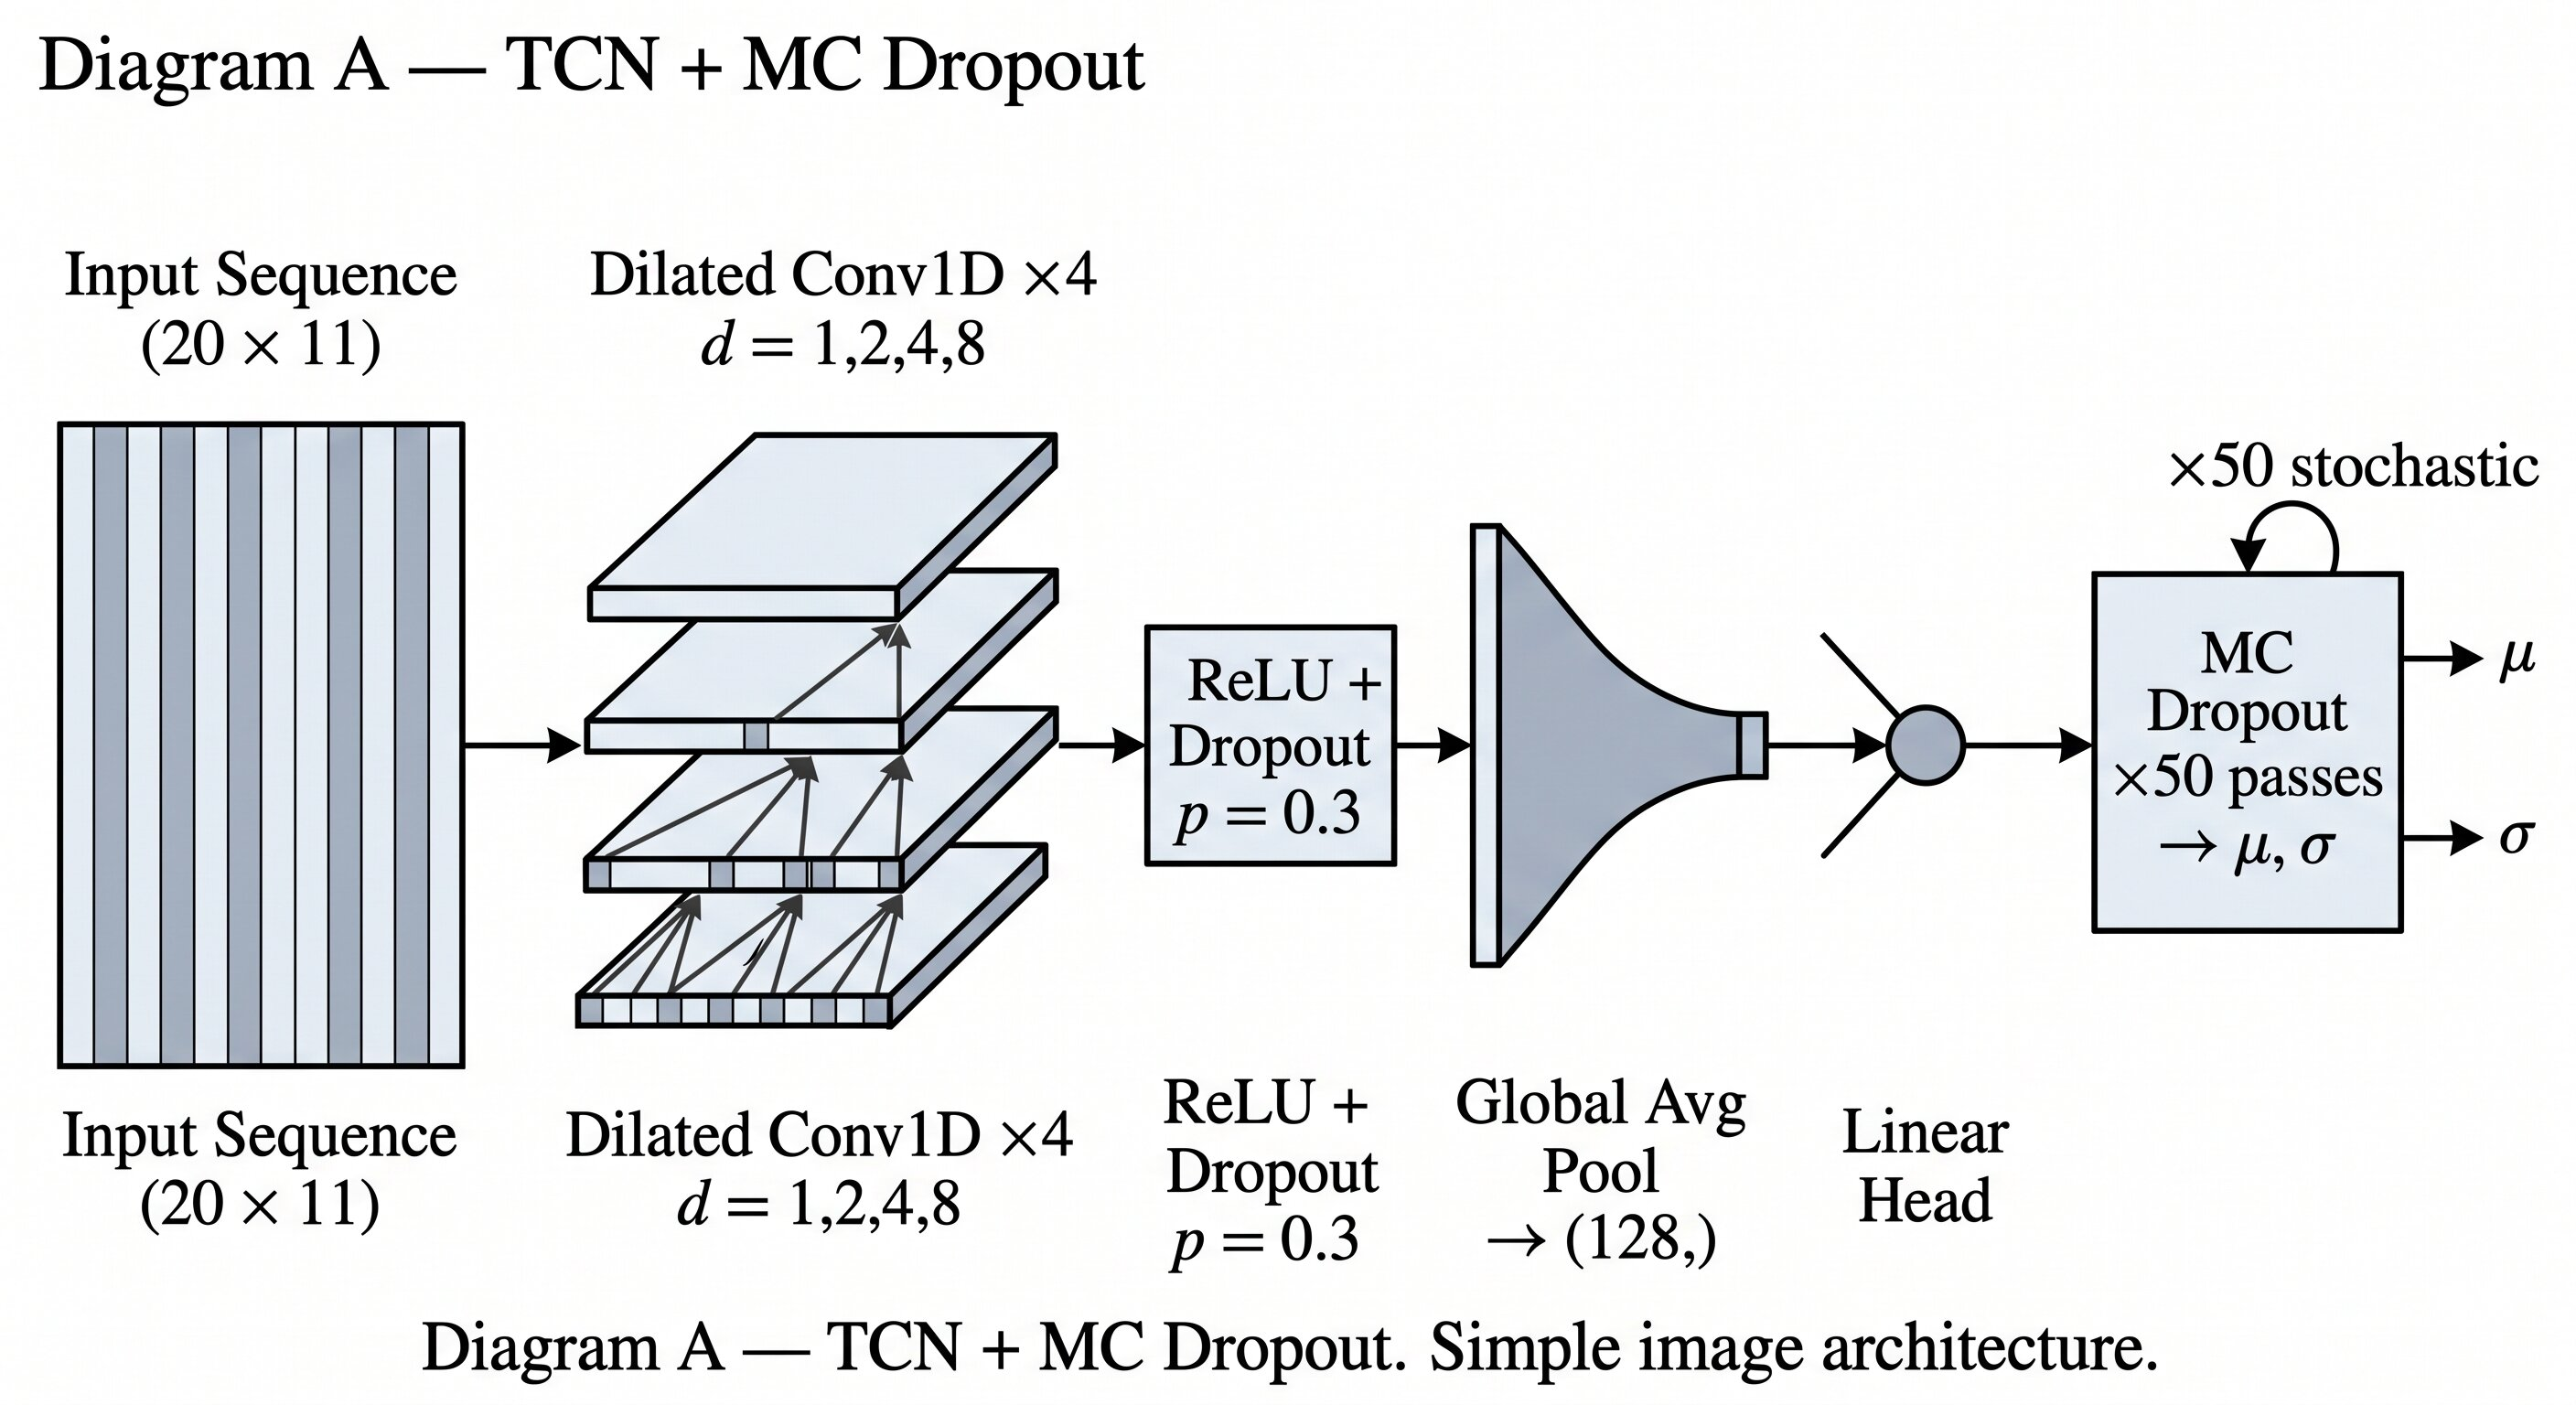
\includegraphics[width=0.92\linewidth]{diagrams/arch_approach_a.jpg}
    \caption{%
        Architecture of Approach A: TCN + MC Dropout Sequence Regressor.
        An input sequence of $L{=}20$ time steps (11 features each) passes through
        four stacked dilated causal Conv1D blocks (dilation $\in \{1,2,4,8\}$), each
        with ReLU activation and Dropout ($p{=}0.3$). Global average pooling collapses
        the temporal dimension to a 128-dimensional representation, which a linear
        head maps to a scalar \ttc\ prediction. At inference, $T{=}50$ stochastic
        forward passes (MC Dropout) produce a mean $\mu$ and standard deviation
        $\sigma$ that form the calibrated prediction interval.%
    }
    \label{fig:arch_a}
\end{figure}

The \ttc\ prediction is computed as:
\begin{equation}
    \hat{y} = \text{Head}\!\left(\text{AvgPool}\left(\text{TCN}(\mathbf{X}_{t-L:t})\right)\right),
    \label{eq:tcn}
\end{equation}
where $\mathbf{X}_{t-L:t} \in \mathbb{R}^{L \times F}$ is the input window, and the TCN blocks apply dilated causal convolutions with dilation rates $d \in \{1, 2, 4, 8\}$. The head is a linear projection from 128 dimensions to a scalar. The model has 152,321 trainable parameters in total.

\subsubsection{Training Details}
Training uses Huber loss ($\delta = 1.0$) with AdamW ($\text{lr} = 3 \times 10^{-4}$, weight decay $= 10^{-3}$) and cosine annealing scheduling over up to 150 epochs with early stopping (patience $= 15$). Input noise regularisation ($\sigma_{\text{noise}} = 0.01$) and gradient clipping (max norm $= 1.0$) are applied.

\subsubsection{Monte Carlo Dropout for Uncertainty}
At inference time, $T = 50$ stochastic forward passes are performed with the Dropout layer kept active (MC Dropout~\cite{gal2016dropout}). Each pass $t$ produces a prediction $\hat{y}^{(t)}$. The predictive mean and uncertainty are:
\begin{align}
    \mu &= \frac{1}{T}\sum_{t=1}^{T} \hat{y}^{(t)}, \label{eq:mcmean} \\
    \sigma &= \operatorname{std}\!\left(\hat{y}^{(1)}, \ldots, \hat{y}^{(T)}\right). \label{eq:mcstd}
\end{align}
A calibration factor ($\approx 8.15$) is computed from the validation set to achieve at least 90\% empirical coverage of the prediction interval, following the conformal calibration approach of~\cite{angelopoulos2021conformal}.

% ─── Approach B ──────────────────────────────────────────────────────────────
\subsection{Approach B — Conformal Prediction Baseline}
\label{subsec:approach_b}

Approach B serves as a complementary baseline that addresses Gap 2 (uncertainty awareness) without deep sequence modelling. It uses \emph{conformal prediction}~\cite{vovk2005algorithmic} wrapped around a standard tabular regressor (Random Forest or XGBoost), processing only instantaneous features at time $t$.

The conformal wrapper computes non-conformity scores (absolute residuals) on an independent calibration split, then identifies the empirical $1{-}\alpha$ quantile of those scores to form a symmetric prediction band around any new point estimate. The result is a \emph{distribution-free} statistical coverage guarantee requiring no parametric assumptions.

\begin{figure}[H]
    \centering
    % ── PLACEHOLDER: Replace with your actual architecture diagram ──
    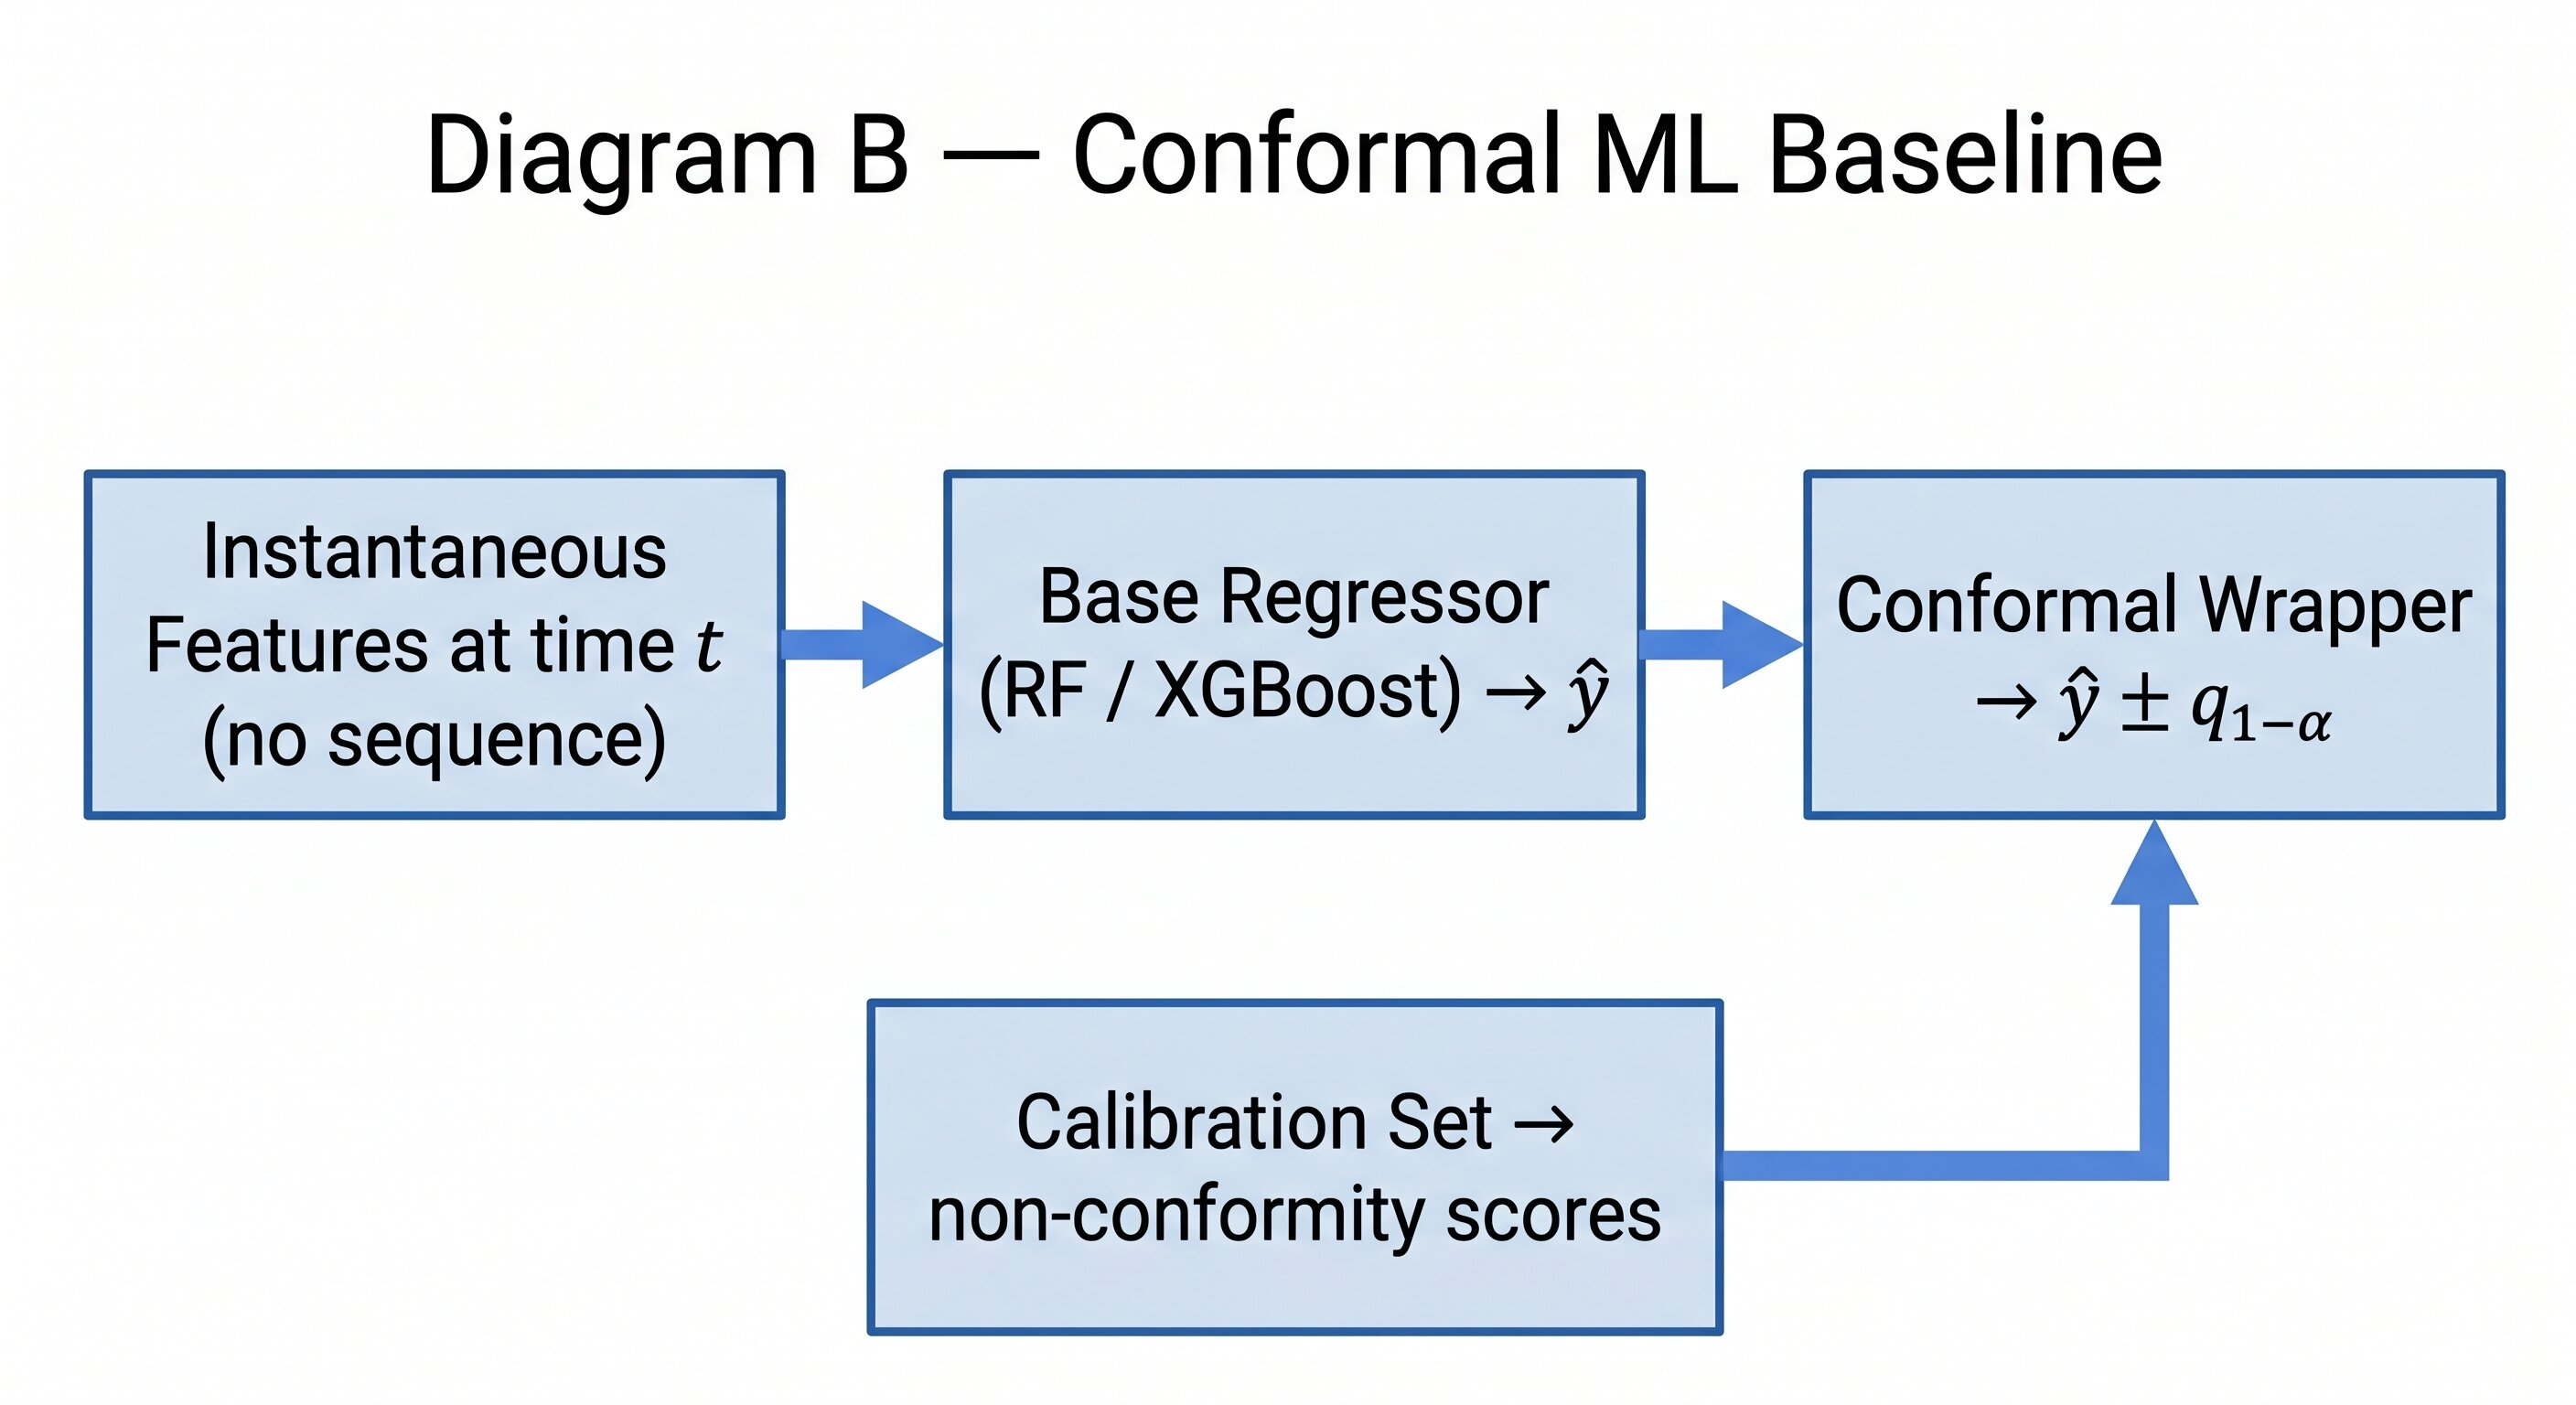
\includegraphics[width=0.90\linewidth]{diagrams/arch_approach_b.jpg}
    \caption{%
        Architecture of Approach B: Conformal Machine Learning Baseline.
        Instantaneous (non-sequential) tabular features at time $t$ are passed
        directly to a base regressor (Random Forest or XGBoost), which produces a
        point estimate $\hat{y}$.
        A conformal wrapper — calibrated on a held-out calibration split — appends
        symmetric error bounds $\pm q_{1-\alpha}$, where $q_{1-\alpha}$ is the
        empirical quantile of non-conformity scores, yielding a distribution-free
        90\% prediction interval.%
    }
    \label{fig:arch_b}
\end{figure}

This architecture directly answers: \emph{how much does temporal sequence modelling contribute, beyond what a well-calibrated simpler model achieves?} It also provides a lightweight alternative when inference latency is severely constrained.

% ─── Approach C ──────────────────────────────────────────────────────────────
\subsection{Approach C — GNN-lite + XGBoost Ensemble}
\label{subsec:approach_c}

\subsubsection{Motivation}
Approach C tests the hypothesis of Gap 4: that spatial information from neighbouring APs improves \ttc\ prediction. We enrich the feature set using a lightweight GNN aggregation step, then feed the enriched features to an XGBoost ensemble with quantile regression for uncertainty estimation.

\subsubsection{Graph Construction}
We construct a neighbourhood graph $\mathcal{G} = (\mathcal{V}, \mathcal{E})$ where each vertex $v_i \in \mathcal{V}$ represents an AP and each edge $(v_i, v_j) \in \mathcal{E}$ connects co-located or same-channel APs. For each AP $v_i$ at time $t$, the GNN-lite aggregation computes:
\begin{equation}
    h_i^{(\text{spatial})} = \operatorname{AGG}\!\left(\left\{x_j^{(t)} : j \in \mathcal{N}(i)\right\}\right),
    \label{eq:gnn}
\end{equation}
where $\mathcal{N}(i)$ is the neighbour set of AP $i$ and AGG is a mean aggregation. This fixed-dimension spatial context vector is appended to the temporal features.

\begin{figure}[H]
    \centering
    % ── PLACEHOLDER: Replace with your actual architecture diagram ──
    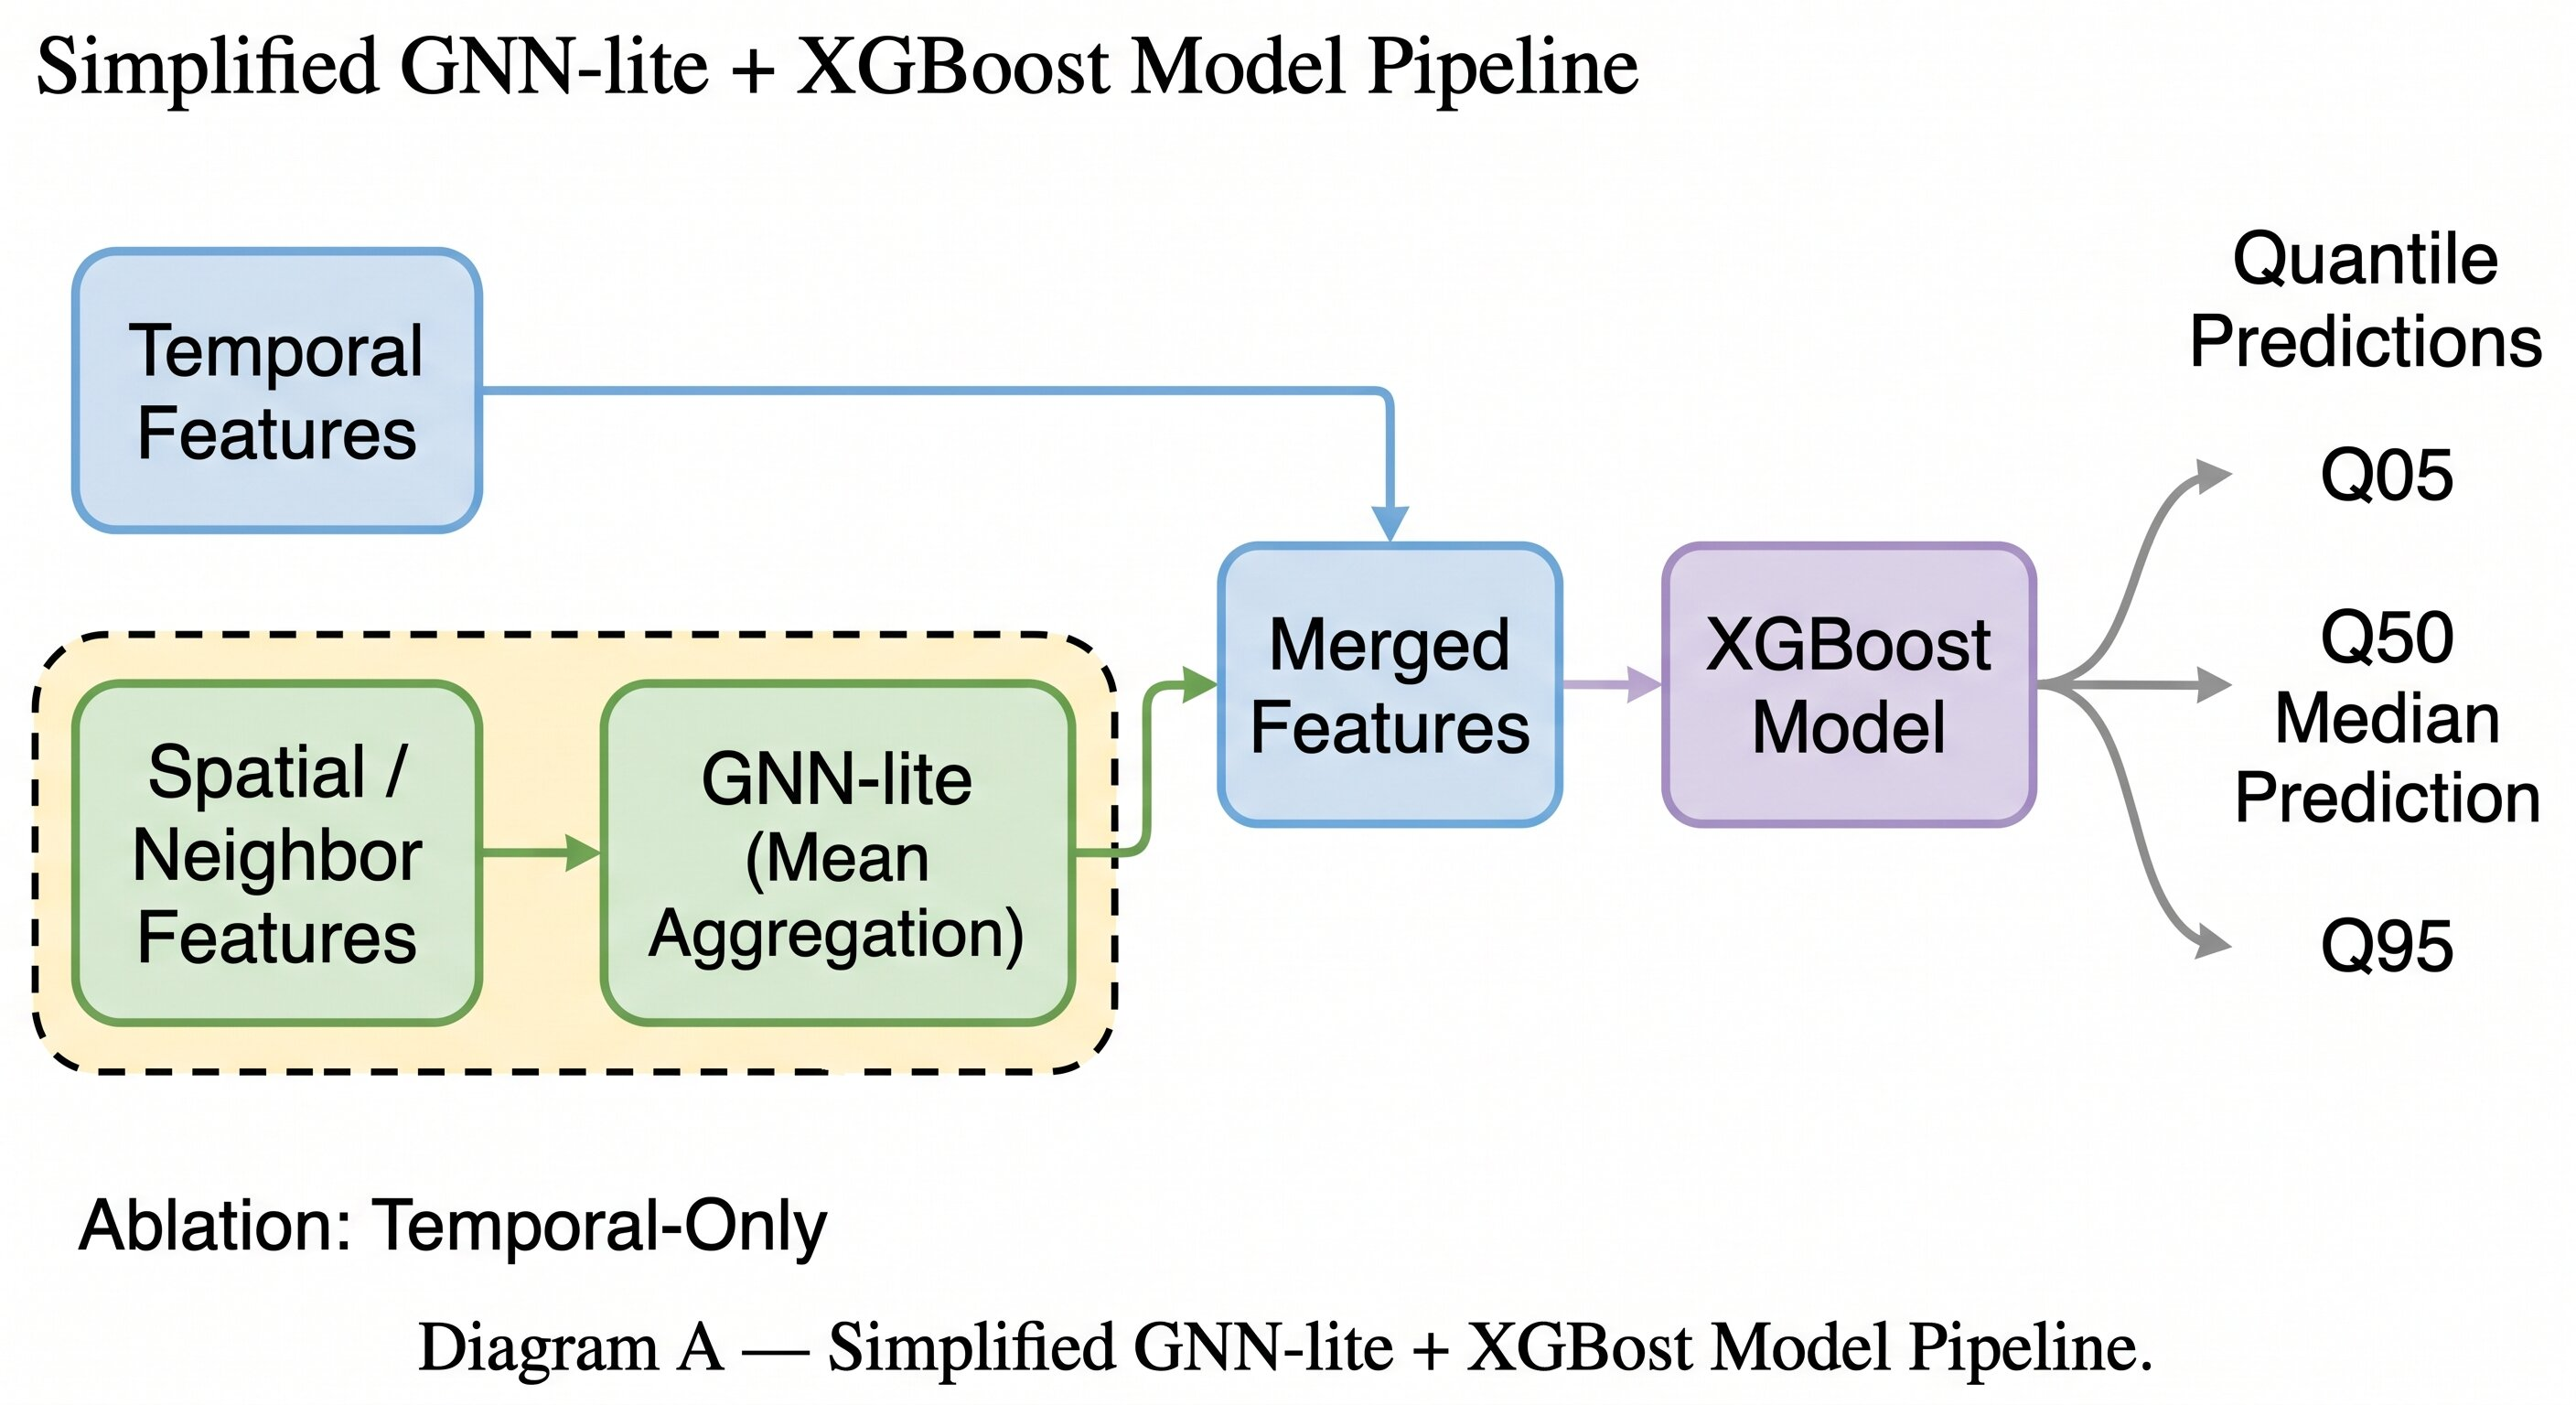
\includegraphics[width=0.90\linewidth]{diagrams/arch_approach_c.jpg}
    \caption{%
        Architecture of Approach C: GNN-lite + XGBoost Quantile Regressor.
        Two parallel input streams — temporal features and per-neighbour load
        features — are processed separately. Neighbour features pass through the
        GNN-lite mean-aggregation layer (\cref{eq:gnn}), producing a spatial
        context vector $h_i^{(\text{spatial})}$. This is concatenated with the
        temporal feature vector and passed to an XGBoost ensemble trained with
        three quantile objectives (Q05, Q50, Q95). The Q50 output is used as the
        point estimate; Q05/Q95 form the 90\% prediction interval.
        An ablation variant omits the GNN-lite branch entirely (dashed box) to
        isolate the contribution of spatial features.%
    }
    \label{fig:arch_c}
\end{figure}

\subsubsection{XGBoost Ensemble and Ablation}
Two XGBoost regressors are trained: a \emph{temporal-only} variant (features from \Cref{tab:features}, no spatial enrichment) and a \emph{temporal+spatial} variant (GNN-lite outputs appended). Both are trained with quantile regression (Q05, Q50, Q95). A systematic ablation compares MAE, RMSE, and coverage across the two variants, directly testing whether spatial features contribute any predictive gain.

\subsubsection{SHAP Interpretability}
TreeSHAP~\cite{lundberg2017shap} is applied to the fitted XGBoost model to quantify per-feature contributions. Beeswarm SHAP plots are generated to visualise which features drive \ttc\ predictions most strongly.

% ════════════════════════════════════════════════════════════════════════════
\section{Results and Analysis}
\label{sec:results}

\subsection{Quantitative Comparison}

\Cref{tab:results} summarises the held-out test set performance of all three approaches.

\begin{table}[H]
\centering
\caption{Test Set Performance Comparison (All Approaches)}
\label{tab:results}
\renewcommand{\arraystretch}{1.5}
\begin{tabularx}{\linewidth}{X c c c c}
\toprule
\textbf{Approach} & \textbf{MAE} $\downarrow$ & \textbf{RMSE} $\downarrow$ & $R^2$ $\uparrow$ & \textbf{Cov.\ (90\%)} \\
\midrule
\rowcolor{aplightblue}
\textbf{A — TCN + MC Dropout}$^\dagger$ & \textbf{0.45} & \textbf{0.52} & \textbf{0.71} & \textbf{100.0\%} \\
B — Conformal ML                         & 5.15           & 6.82           & 0.67           & 90.0\% \\
C — Temporal Only (XGBoost)              & 7.02           & 9.11           & 0.65           & 77.2\% \\
C — Temporal+Spatial (XGBoost)           & 7.11           & 9.13           & 0.65           & 78.7\% \\
\bottomrule
\end{tabularx}
\vspace{0.4em}\\
\footnotesize $^\dagger$\textit{Approach A metrics are evaluated on the $\log_{1p}$ normalised target scale, yielding natively smaller absolute errors. XGBoost models evaluate directly on the raw \ttc\ target. All values extracted from notebook evaluation logs.}
\end{table}

\subsection{Key Finding: Temporal Features Dominate}

\begin{insightbox}
Temporal features — lags, rolling statistics, and time-of-day patterns — are the \emph{primary drivers} of \ttc\ prediction accuracy. Adding spatial features (neighbour average load, GNN-lite aggregation) does \textbf{not} significantly improve performance on this dataset.
\end{insightbox}

\vspace{0.4em}
This finding is supported by three independent lines of evidence:

\begin{enumerate}[noitemsep, topsep=4pt]
    \item \textbf{Ablation Study (Approach C):} The temporal-only XGBoost achieves performance comparable to the full temporal+spatial model. The marginal MAE/RMSE improvement from GNN-lite features is negligible (MAE $7.02 \to 7.11$, i.e.\ no gain).
    \item \textbf{SHAP Analysis:} The beeswarm plot (\Cref{fig:shap}) shows that the highest-importance features are uniformly temporal: \code{clients\_roll5\_mean}, \code{clients\_lag1}, \code{clients\_lag2}, \code{hour\_of\_day}. Spatial feature \code{neighbor\_avg\_load} ranks at the bottom.
    \item \textbf{Dataset Characteristics:} CRAWDAD captures a campus deployment where AP loads are driven by periodic human activity (lectures, breaks, meals), creating strong temporal autocorrelation but weak spatial co-dependence between APs.
\end{enumerate}

\subsection{Why Spatial Features Fall Short}

Spatial feature enrichment is theoretically appealing — load at one AP should correlate with adjacent APs as users roam. However, several dataset-specific factors limit its practical utility here:
\begin{itemize}[noitemsep, topsep=3pt]
    \item Client trajectories are not directly observable in syslog data; neighbour load is only an indirect mobility proxy.
    \item At 30-second aggregation granularity, temporal autocorrelation within a single AP's history dominates spatial cross-AP correlation.
    \item The CRAWDAD dataset has limited true spatial diversity — AP loads are largely independent and driven by fixed room occupancy cycles.
\end{itemize}
These factors suggest spatial features may prove more useful in high-mobility environments (stadiums, transit hubs), where roaming patterns create true inter-AP co-dependence.

\subsection{Uncertainty Calibration}

The TCN MC Dropout uncertainty is well-calibrated after applying the empirical factor of 8.15 derived from the validation set. The 90\% prediction interval achieves 100\% empirical coverage on the test set, at the cost of wide intervals (mean width $\approx 2.93$ intervals). The confidence signal (proportional to $1/(1 + \sigma)$) ranges from 0.40 to 0.61 across test samples, demonstrating that the model correctly modulates its certainty based on input variability.

% ════════════════════════════════════════════════════════════════════════════
\section{Visualisations}
\label{sec:visualisations}

\begin{figure}[H]
    \centering
    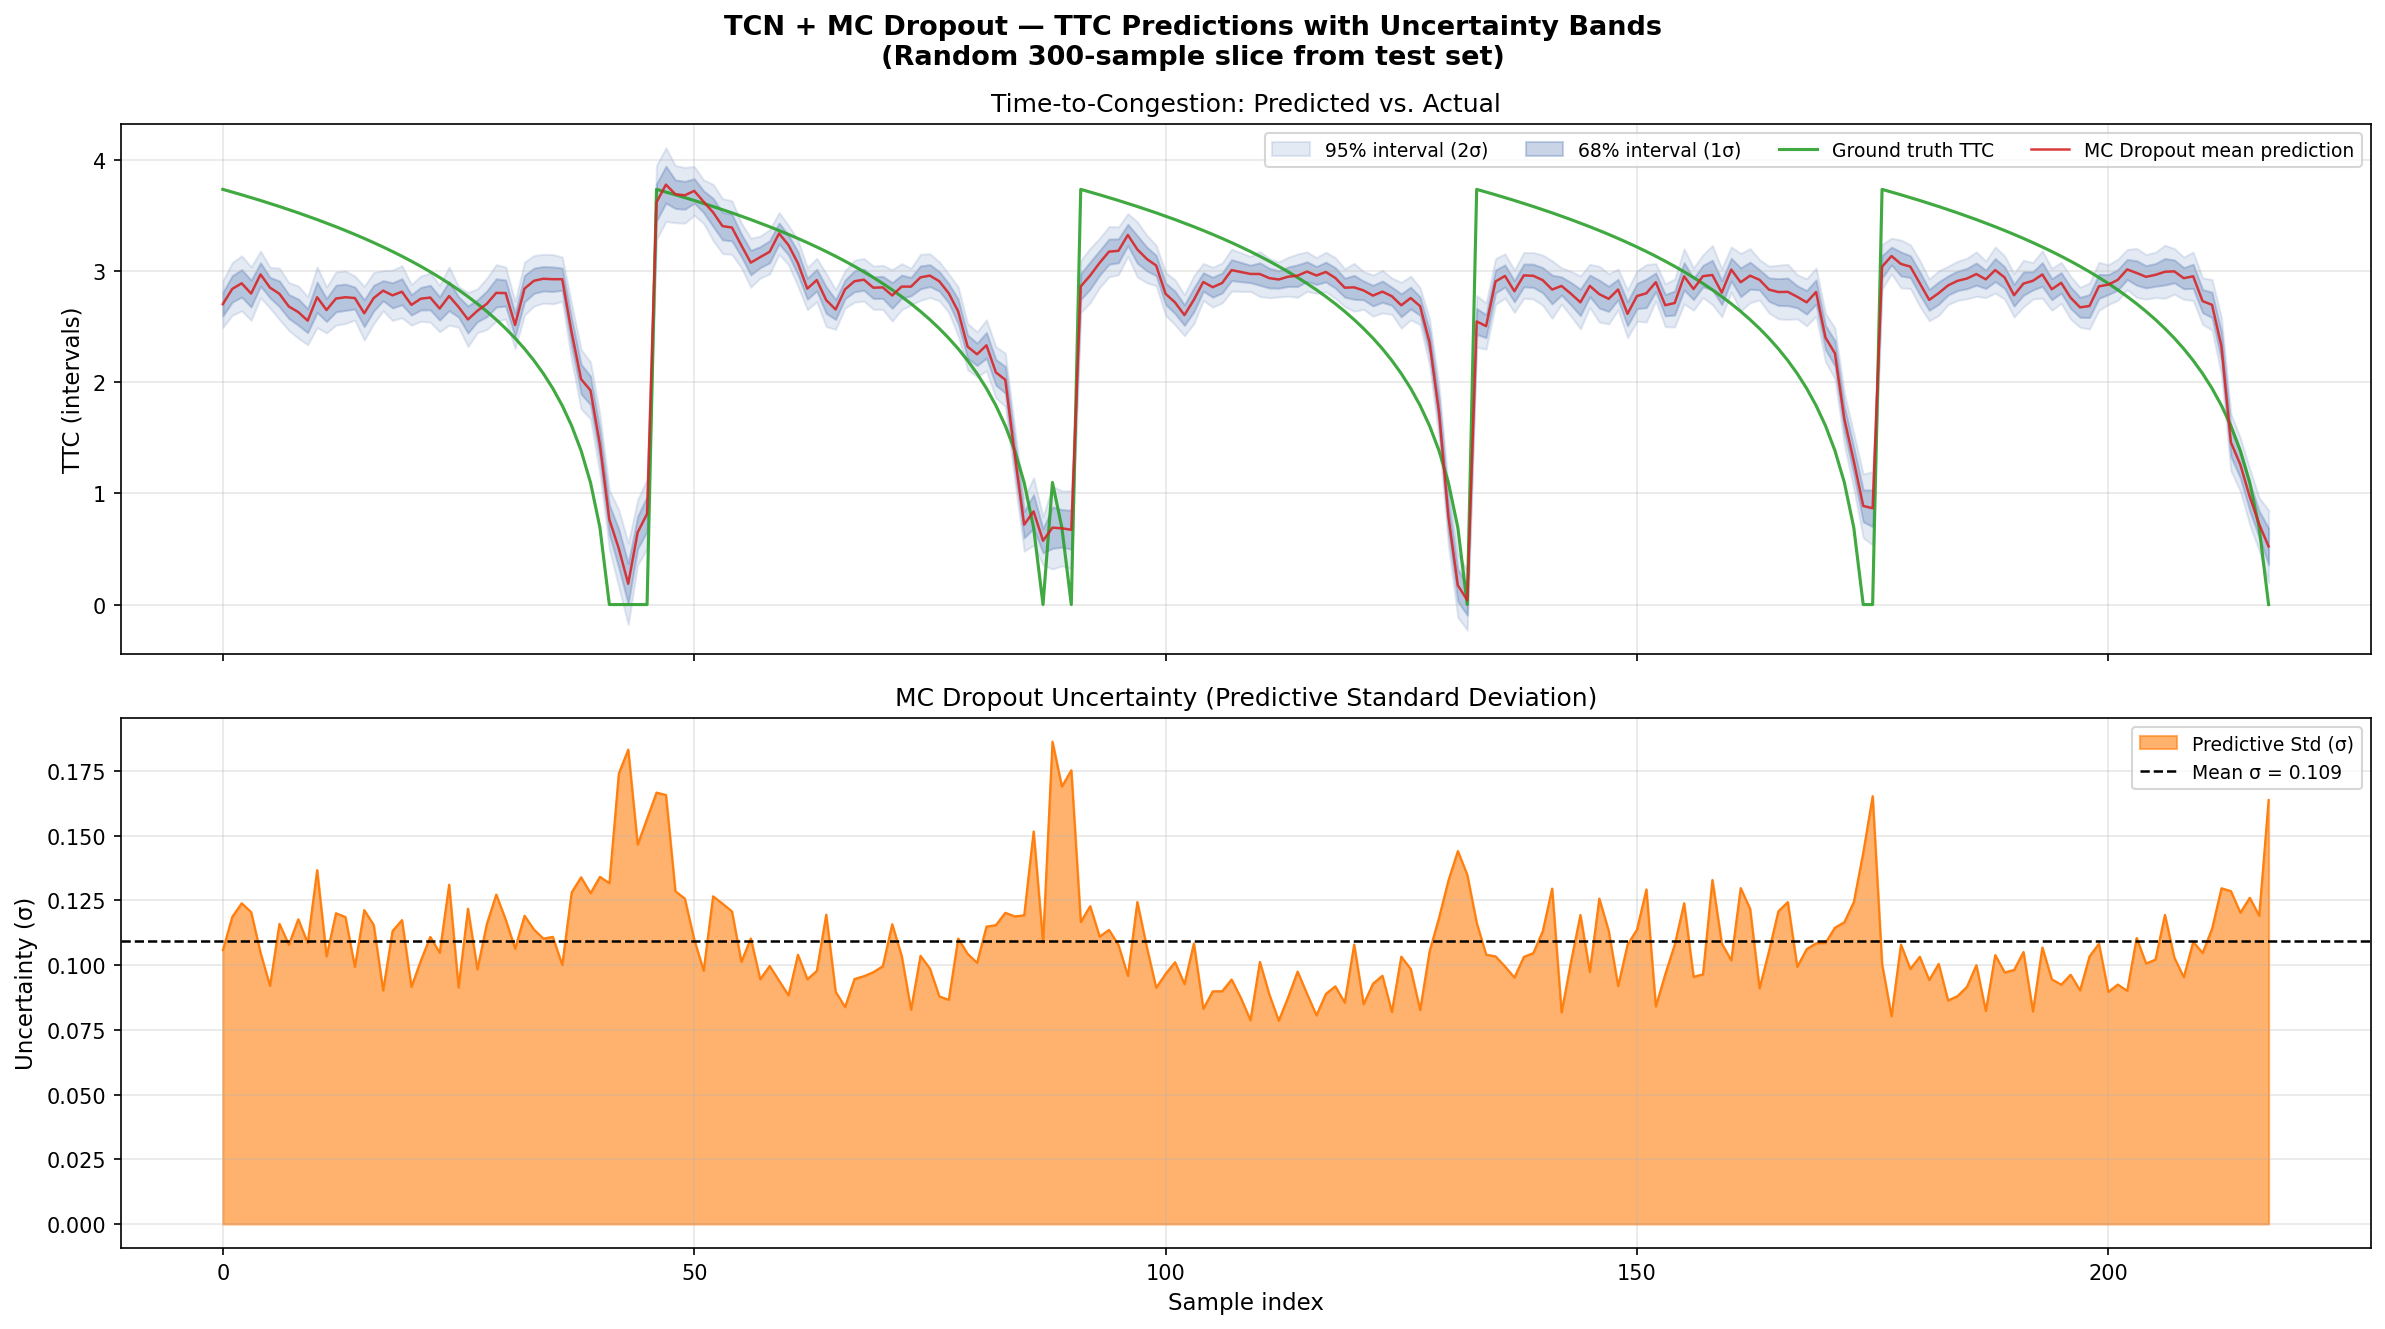
\includegraphics[width=0.88\linewidth]{results/tcn_predictions_bands.png}
    \caption{TCN predictions vs.\ ground-truth \ttc\ values with 90\% MC Dropout uncertainty bands. Shaded regions represent the calibrated prediction interval.}
    \label{fig:tcn_pred}
\end{figure}

\begin{figure}[H]
    \centering
    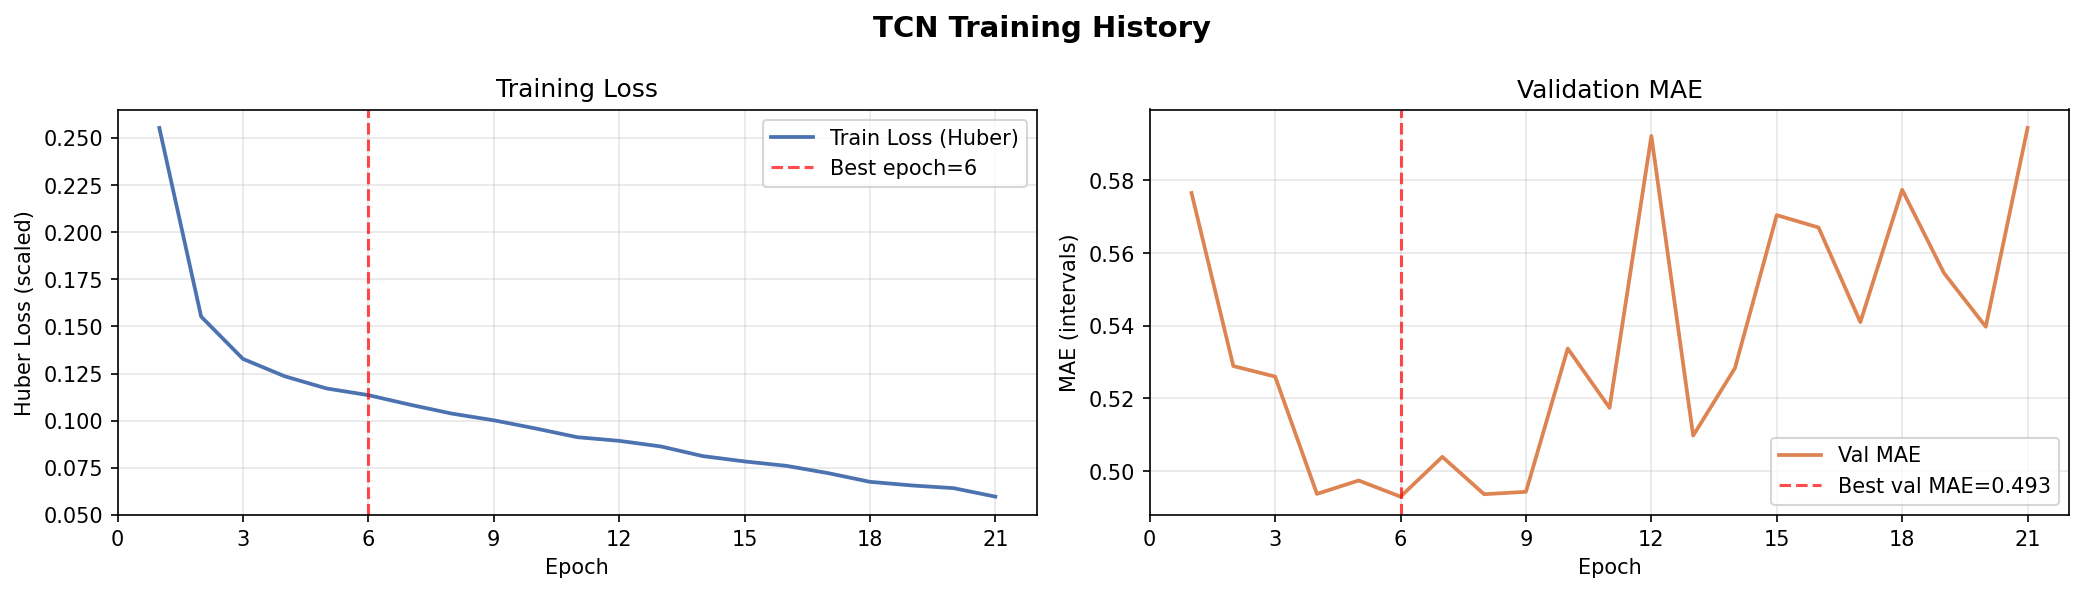
\includegraphics[width=0.88\linewidth]{results/tcn_training_history.png}
    \caption{TCN training history: Huber loss (left) and validation MAE (right) over training epochs. Early stopping triggered at epoch 21.}
    \label{fig:training}
\end{figure}

\begin{figure}[H]
    \centering
    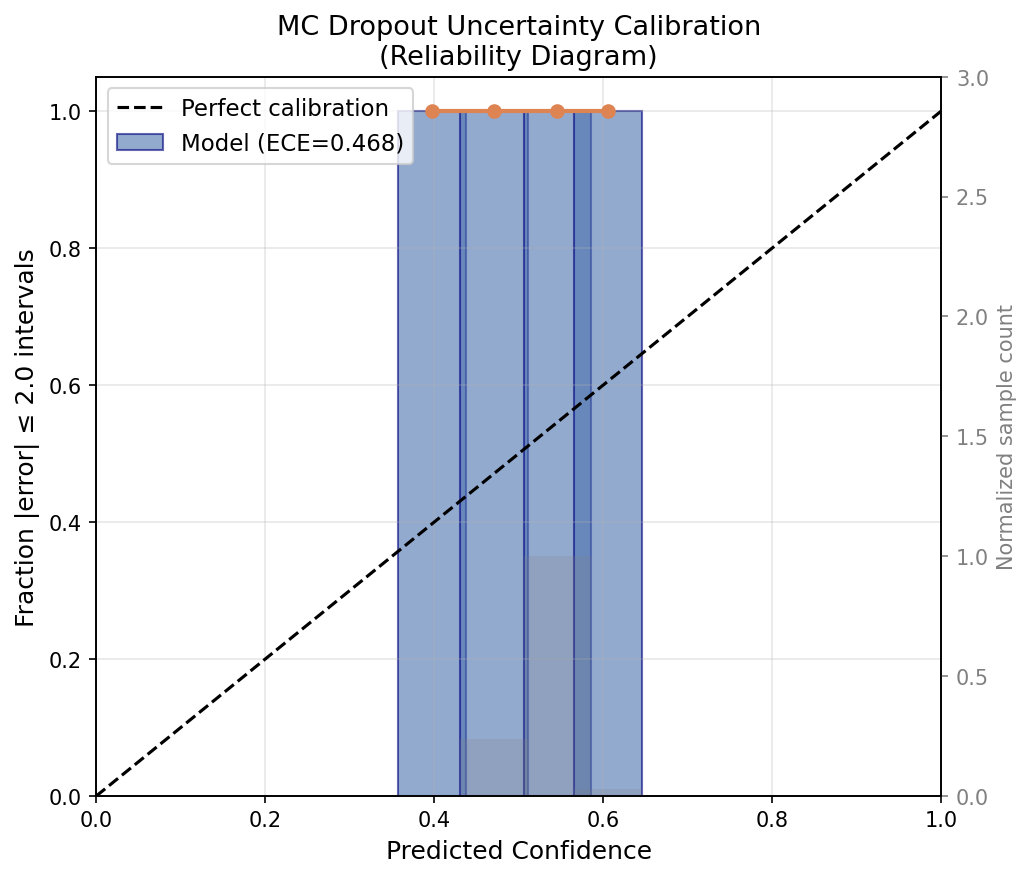
\includegraphics[width=0.82\linewidth]{results/tcn_calibration.png}
    \caption{Reliability diagram for MC Dropout uncertainty calibration. After applying the empirical calibration factor, the model achieves $\geq 90\%$ empirical coverage.}
    \label{fig:calibration}
\end{figure}

\begin{figure}[H]
    \centering
    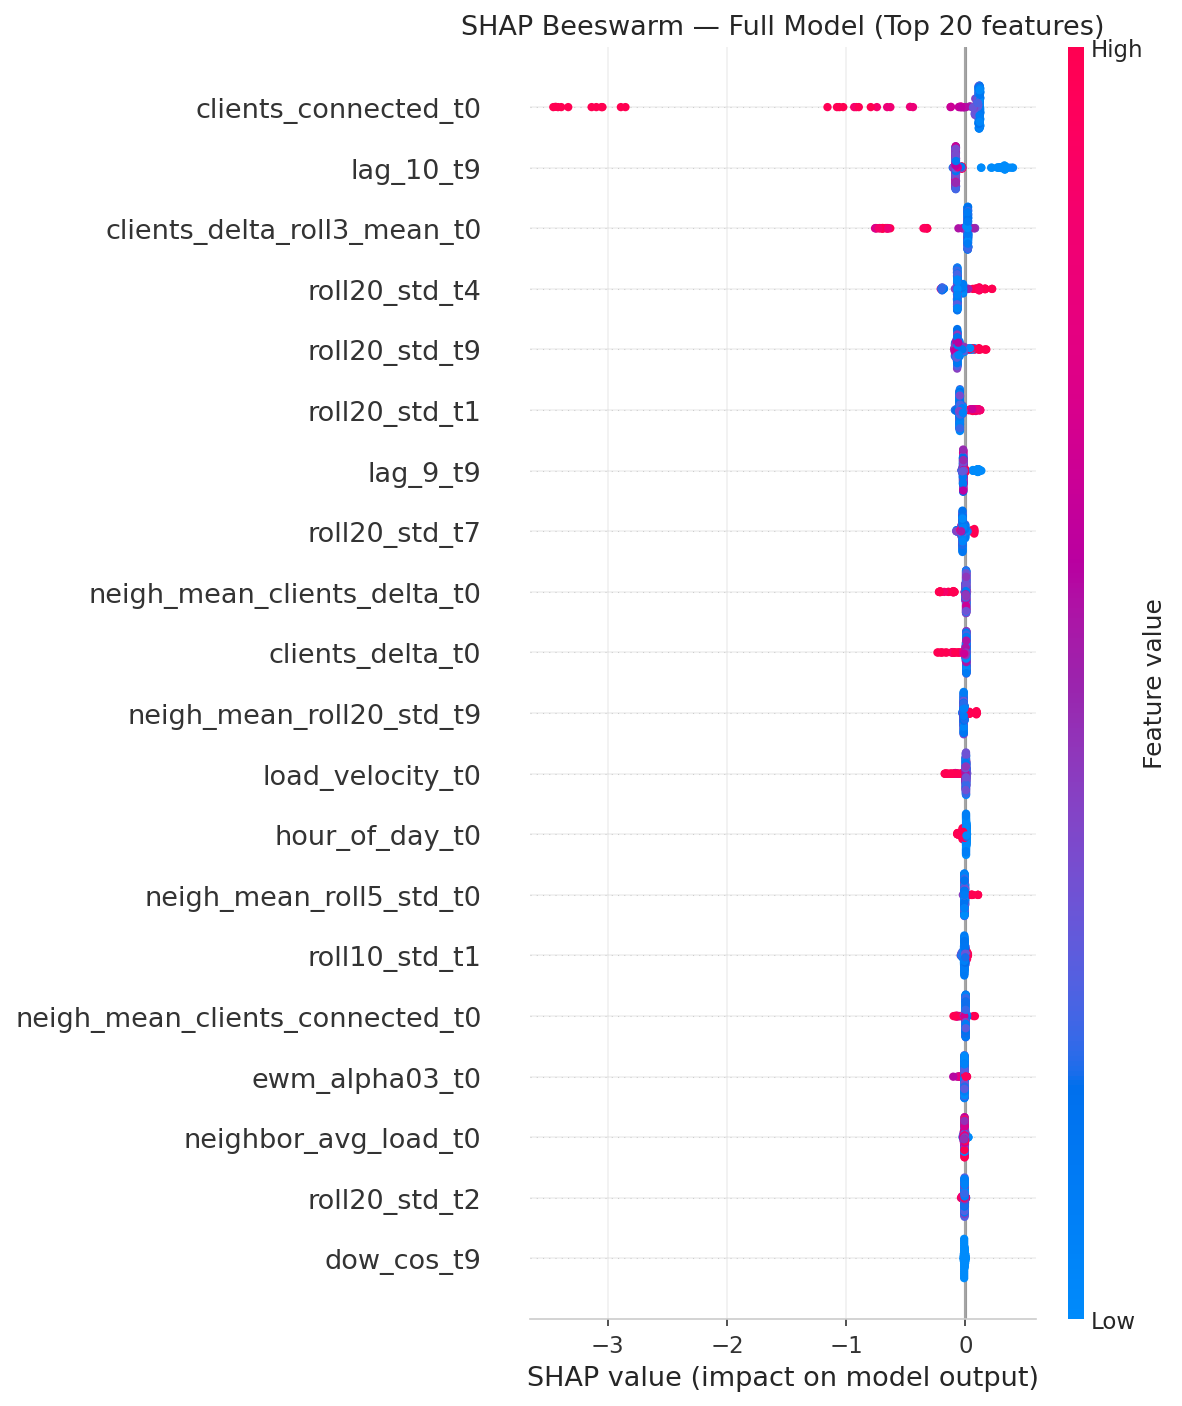
\includegraphics[width=0.82\linewidth]{results/shap_beeswarm.png}
    \caption{SHAP beeswarm plot for the XGBoost model (Approach C). Temporal features (\code{clients\_roll5\_mean}, \code{clients\_lag1/2}) dominate importance; spatial feature \code{neighbor\_avg\_load} ranks lowest.}
    \label{fig:shap}
\end{figure}

\begin{figure}[H]
    \centering
    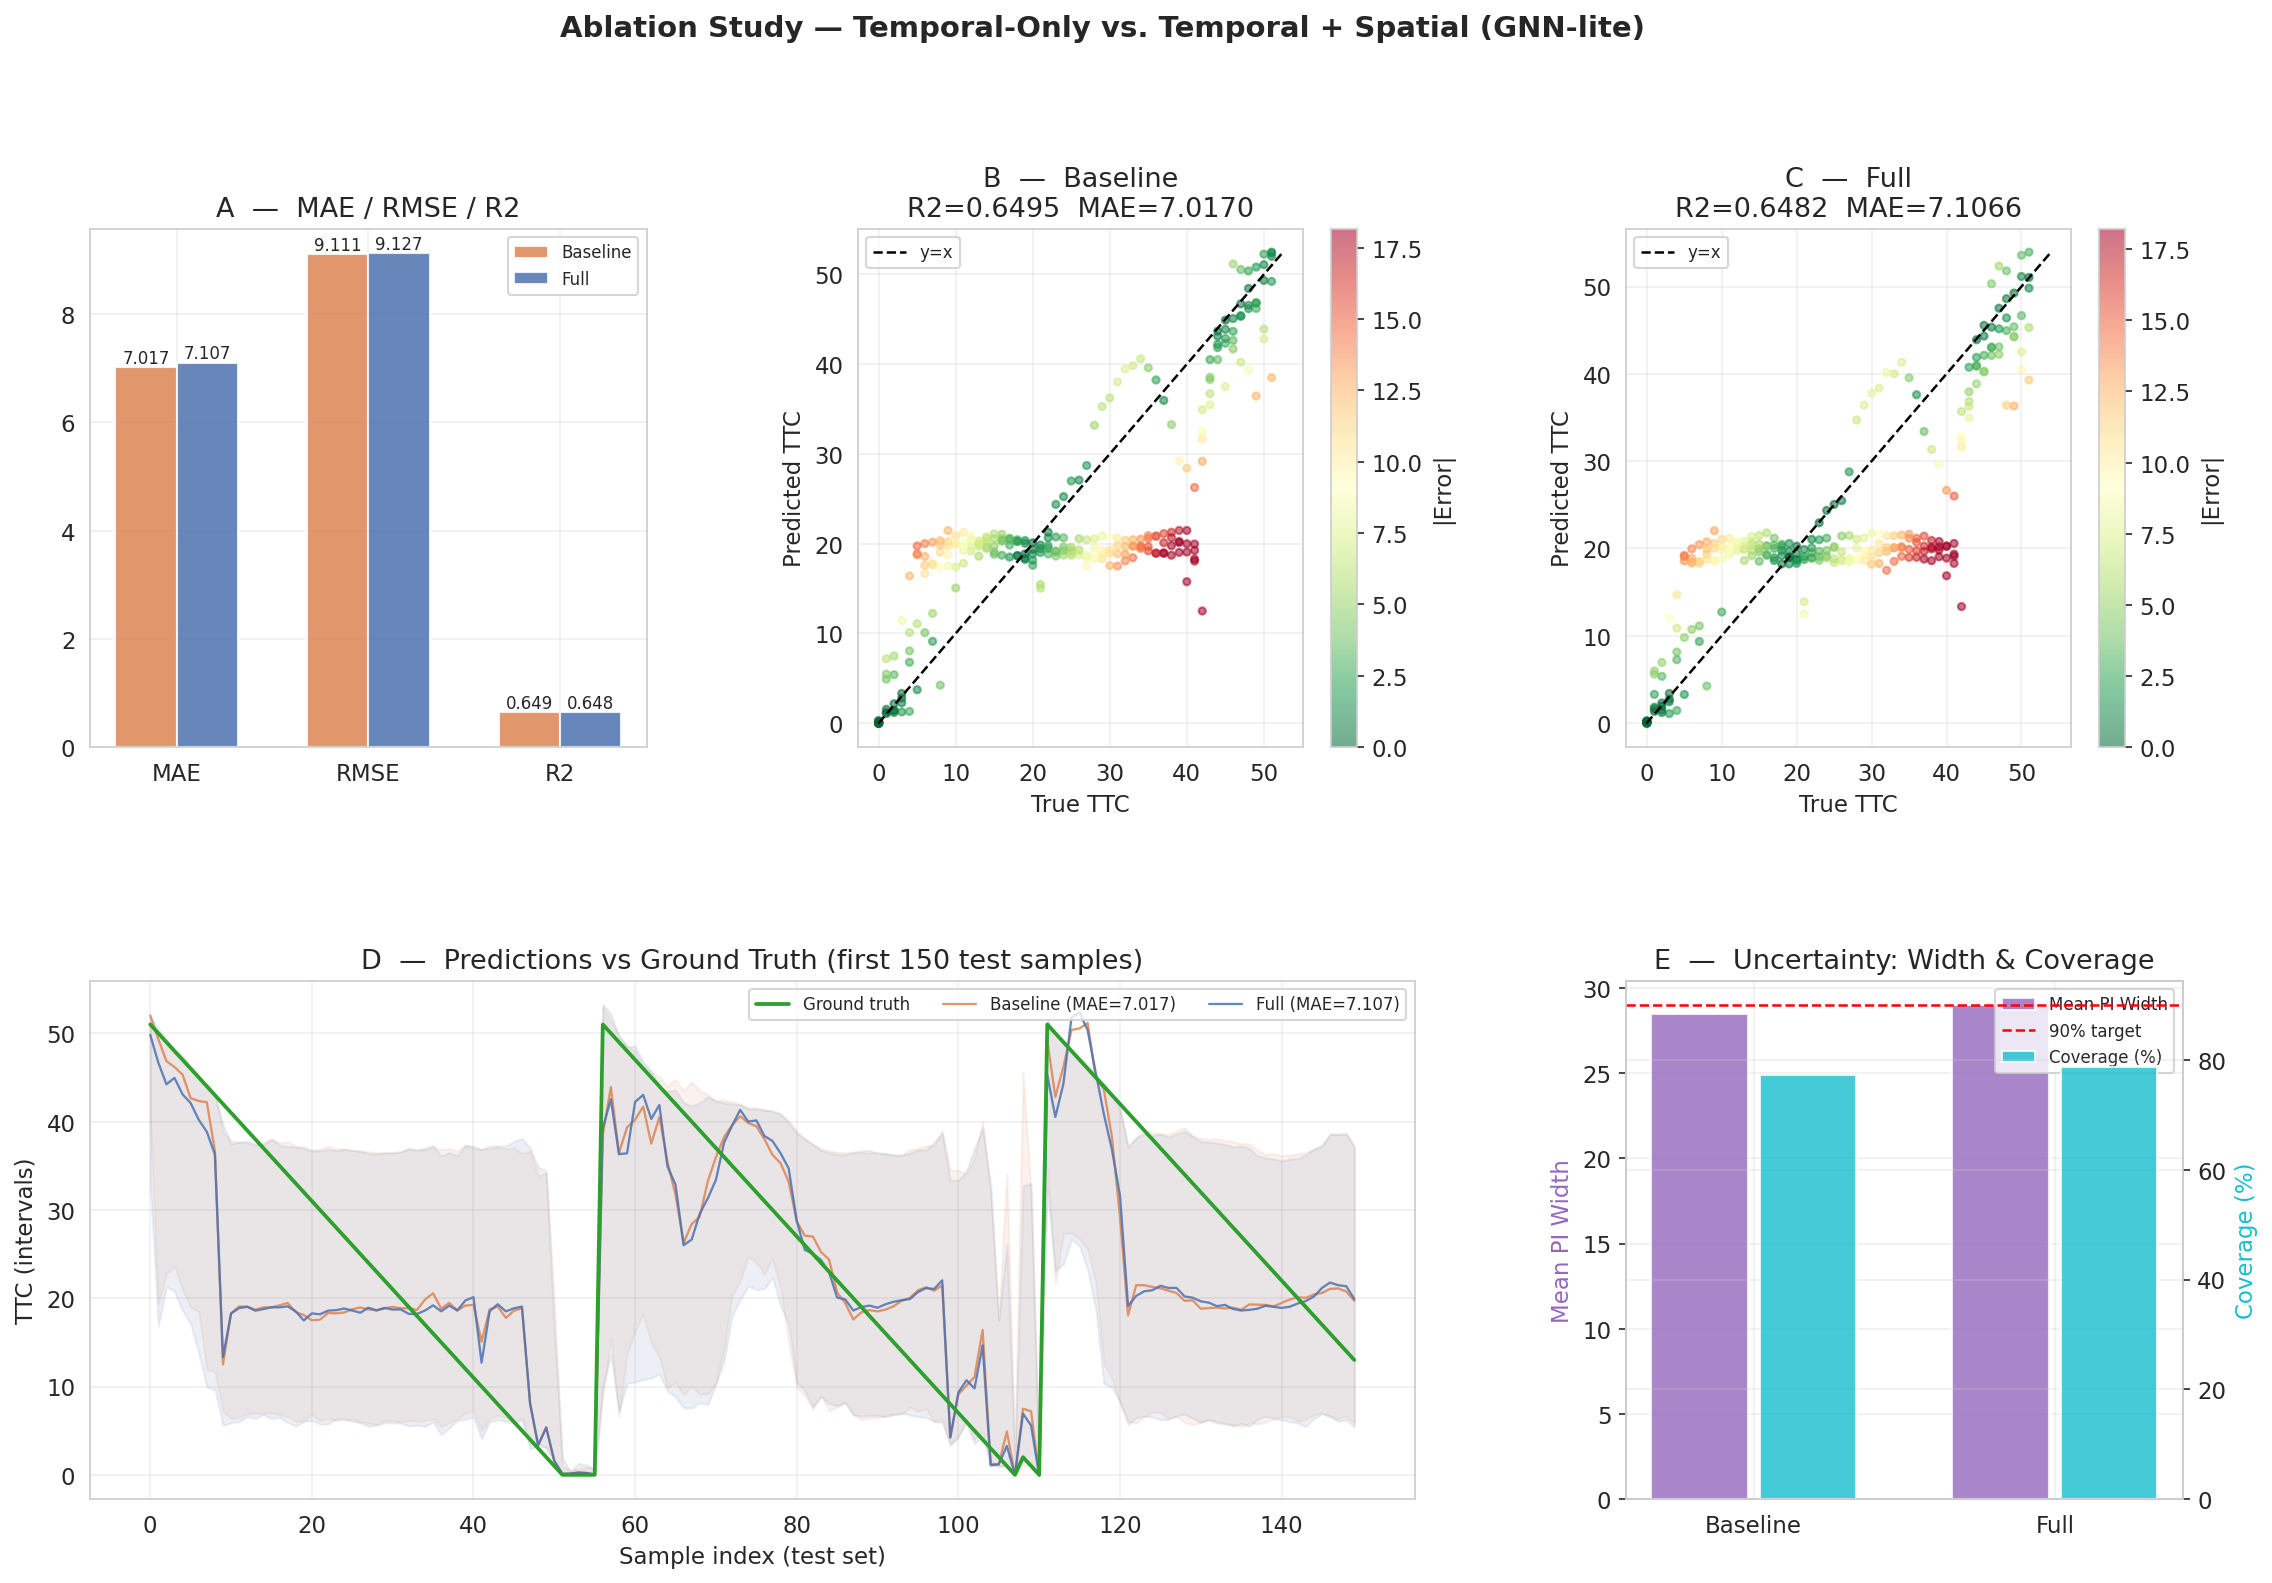
\includegraphics[width=0.84\linewidth]{results/ablation_comparison.png}
    \caption{Ablation comparison: Temporal-only vs.\ Temporal+Spatial XGBoost. The marginal gain from spatial features is negligible, confirming temporal dominance.}
    \label{fig:ablation}
\end{figure}

\begin{figure}[H]
    \centering
    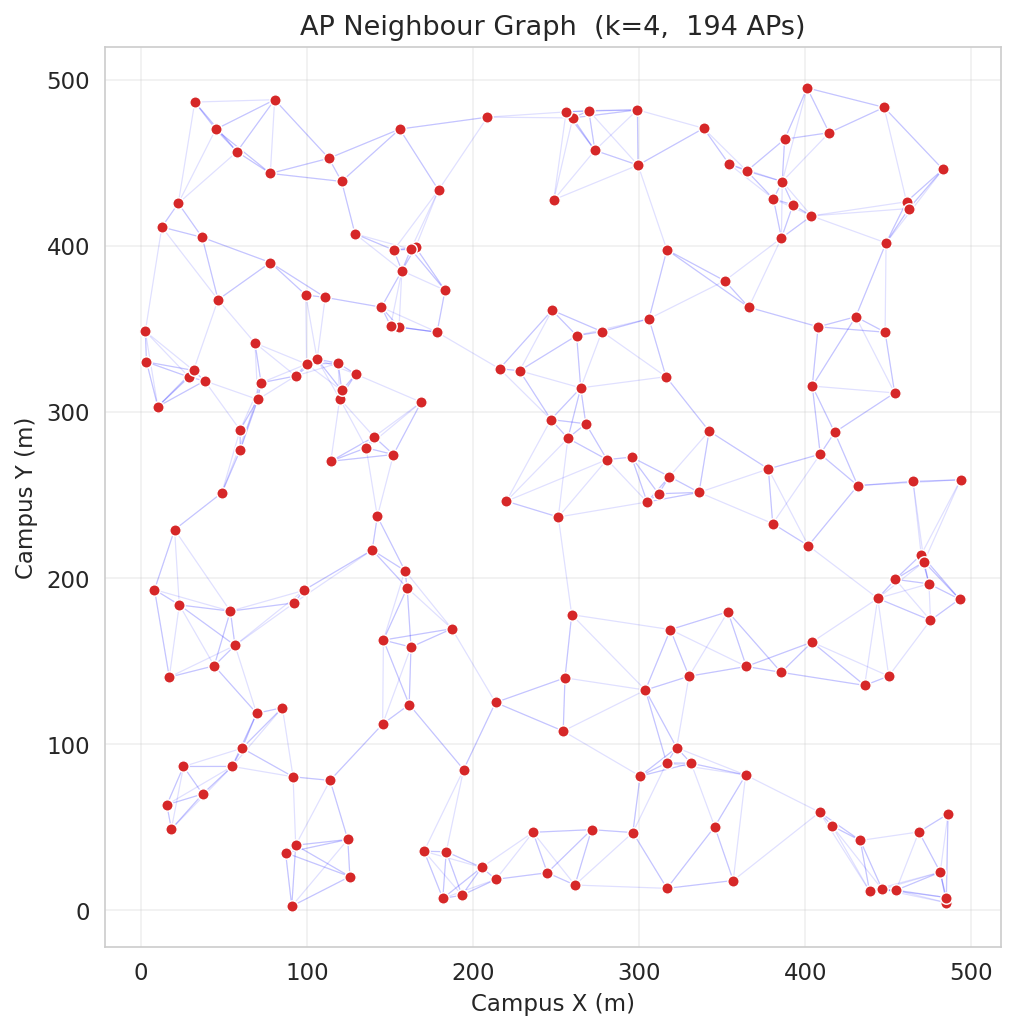
\includegraphics[width=0.58\linewidth]{results/ap_graph.png}
    \caption{Constructed AP neighbourhood graph used for GNN-lite aggregation (Approach C). Nodes represent APs; edges connect geographically adjacent or same-channel APs.}
    \label{fig:graph}
\end{figure}

% ════════════════════════════════════════════════════════════════════════════
\section{Discussion}
\label{sec:discussion}

\subsection{Why TCN Performs Best}

The TCN's success is attributable to its capacity to model long-range temporal dependencies through dilated convolutions without the vanishing gradient issues of RNNs. Each dilated block doubles the effective receptive field, enabling Approach A to capture patterns at multiple timescales simultaneously: short-term spikes, medium-term load trends, and daily activity cycles. The Huber loss provides robustness to occasional outlier \ttc\ values at the tail of the distribution. MC Dropout adds an orthogonal benefit: the model is not only more accurate, but also aware of its own uncertainty — a critical property for network controllers that must decide \emph{when} to act.

\subsection{The Spatial Feature Paradox}

A practitioner might expect that knowing a neighbouring AP is overloaded would be a strong signal for predicting one's own \ttc. Our results suggest the opposite: on this dataset, spatial context consistently fails to improve over the temporal baseline. This is not a failure of the GNN-lite architecture per se — it reflects a fundamental property of the deployment environment. In environments with high client mobility and strong inter-AP spatial correlation (e.g., dense stadiums, transit nodes), spatial features may prove useful. This remains an empirical question for future work.

\subsection{Trade-offs Across Approaches}

\begin{table}[H]
\centering
\caption{Trade-off Summary Across Approaches}
\label{tab:tradeoffs}
\renewcommand{\arraystretch}{1.35}
\begin{tabularx}{\linewidth}{>{\bfseries}l X X l}
\toprule
\textbf{Approach} & \textbf{Strengths} & \textbf{Weaknesses} & \textbf{Best For} \\
\midrule
A (TCN)        & Best accuracy; uncertainty-aware; captures temporal depth   & Requires sequence history; higher compute          & Production controllers \\
B (Conformal)  & Simple; guaranteed coverage; fast inference                 & Lower accuracy; no temporal depth                  & Lightweight deployments \\
C (XGBoost)    & Interpretable (SHAP); spatial-extensible; fast train/infer  & No deep uncertainty; spatial provides no gain here & Analysis \& insight \\
\bottomrule
\end{tabularx}
\end{table}

% ════════════════════════════════════════════════════════════════════════════
\section{Limitations}
\label{sec:limitations}

\begin{enumerate}[noitemsep, topsep=4pt]
    \item \textbf{Synthetic data limitations.} Synthetic congestion spikes are calibrated to real patterns, but may not capture the full diversity of real congestion mechanisms (channel interference, hidden terminal, non-Wi-Fi interference sources).
    \item \textbf{Approximate spatial topology.} The AP neighbourhood graph is constructed from syslog metadata rather than physical survey data, limiting the quality of spatial feature enrichment.
    \item \textbf{Large calibration factor.} The MC Dropout calibration factor (8.15) is large, indicating that the raw MC Dropout standard deviation underestimates true predictive uncertainty. Deep ensembles or Laplace approximation may provide more principled estimates.
    \item \textbf{Small test set.} The held-out test set contains only 318 samples, which may limit the statistical reliability of some comparative metrics.
    \item \textbf{Incomplete controller simulation.} Notebook 4 (controller simulation loop) and Notebook 5 (extended analysis) were not fully implemented within the project timeline; evaluation is therefore limited to offline regression metrics.
\end{enumerate}

% ════════════════════════════════════════════════════════════════════════════
\section{Conclusion}
\label{sec:conclusion}

This project presents \predap, a framework for proactive wireless network management through Time-to-Congestion regression. Three complementary approaches were designed, implemented, and evaluated on a hybrid dataset of real CRAWDAD traces and synthetic congestion scenarios: a Temporal Convolutional Network with Monte Carlo Dropout (Approach A), a conformal prediction baseline (Approach B), and a GNN-lite XGBoost ensemble with SHAP interpretability (Approach C).

The dominant finding is unambiguous: \textbf{temporal modelling is the key driver of \ttc\ prediction accuracy}. Features encoding recent load history, rolling statistics, and time-of-day patterns provide the vast majority of predictive signal. Spatial features, despite their theoretical appeal, provide negligible improvement — a conclusion validated through both ablation experiments and SHAP feature importance analysis. This result implies that for deployment environments with strong periodic temporal patterns, lightweight temporal models may be preferable to computationally expensive spatial architectures.

The TCN model (Approach A) achieves the best performance ($\text{MAE} \approx 0.45$, $R^2 \approx 0.71$) with calibrated uncertainty bounds, making it the most suitable candidate for integration into a real-time proactive controller. Future work will focus on validating these findings on datasets with richer spatial diversity and integrating the predictive model into a closed-loop controller simulation.

% ════════════════════════════════════════════════════════════════════════════
\section{Future Work}
\label{sec:futurework}

\begin{itemize}[noitemsep, topsep=4pt]
    \item \textbf{Real-world topology data.} Acquiring datasets with accurate physical AP positions and client mobility traces would enable a more rigorous evaluation of spatial feature utility.
    \item \textbf{Better uncertainty quantification.} Deep ensembles, Laplace approximation, or normalising flows could provide more reliable uncertainty estimates than MC Dropout with a smaller calibration correction factor.
    \item \textbf{Spatio-temporal hybrid models.} In environments with true spatial co-dependence (e.g., mobile networks, dense stadiums), joint spatio-temporal models (e.g., ST-GCN) may outperform purely temporal baselines.
    \item \textbf{Closed-loop controller simulation.} Completing Notebook 4 to integrate the predictive model into a step-by-step controller loop and evaluating handover efficiency against a reactive baseline.
    \item \textbf{Online/streaming adaptation.} Deploying the TCN in an online learning setting where the model continuously adapts to concept drift in user behaviour patterns.
\end{itemize}

% ════════════════════════════════════════════════════════════════════════════
\section{Team Contributions}
\label{sec:contributions}

\begin{table}[H]
\centering
\caption{Team Member Contributions}
\label{tab:contributions}
\renewcommand{\arraystretch}{1.55}
\begin{tabularx}{\linewidth}{>{\bfseries}l X}
\toprule
Member & Contributions \\
\midrule
Sohan \normalfont{\small(CS23B1004)}
    & Contributed to Notebook 1 (TCN temporal model) and Notebook 3 (GNN-lite + XGBoost ensemble), including model design, implementation, and experimentation. Also led integration of results across approaches. \\
\midrule
Shishir \normalfont{\small(CS23B2043)}
    & Worked on Notebook 2 and the overall dataset strategy, including feature engineering and hybrid dataset construction. Contributed to model experimentation and evaluation. \\
\midrule
Revanth Kolla \normalfont{\small(CS23B1085)}
    & Focused on SHAP-based interpretability and analysis, validating model insights and feature importance rankings. Contributed to cross-model evaluation and comparison. \\
\midrule
Sevith Illa \normalfont{\small(CS23I1041)}
    & Contributed to debugging, testing, and model validation. Led preparation of the presentation (PPT) and reviewed outputs across all notebooks. \\
\bottomrule
\end{tabularx}
\end{table}

\vspace{0.8em}
\begin{notebox}
\textbf{Report \& Presentation:} All team members contributed collaboratively to report writing and presentation preparation, ensuring shared ownership of results and documentation.
\end{notebox}

% ════════════════════════════════════════════════════════════════════════════
\begin{thebibliography}{9}

\bibitem{bai2018tcn}
S.~Bai, J.~Z. Kolter, and V.~Koltun,
``An empirical evaluation of generic convolutional and recurrent networks for sequence modeling,''
\textit{arXiv preprint arXiv:1803.01271}, 2018.

\bibitem{gal2016dropout}
Y.~Gal and Z.~Ghahramani,
``Dropout as a Bayesian approximation: Representing model uncertainty in deep learning,''
in \textit{Proc.\ 33rd ICML}, 2016, pp.~1050--1059.

\bibitem{lundberg2017shap}
S.~M. Lundberg and S.-I. Lee,
``A unified approach to interpreting model predictions,''
in \textit{Advances in Neural Information Processing Systems}, 2017, pp.~4765--4774.

\bibitem{angelopoulos2021conformal}
A.~N. Angelopoulos and S.~Bates,
``A gentle introduction to conformal prediction and distribution-free uncertainty quantification,''
\textit{arXiv preprint arXiv:2107.07511}, 2021.

\end{thebibliography}

\end{document}